%% ADScAI 2026 — Revised submission
%% Authors: S.V. Chanupa Hansaja & W.G. Kusal Pabasara

\documentclass[sigconf]{acmart}

% --- Rights management (ADScAI override) ---
\setcopyright{none}
\settopmatter{printacmref=false}

\AtBeginDocument{%
  \providecommand\BibTeX{{%
    Bib\TeX}}}

\acmConference[ADScAI Conference]{Second Annual Conference of Department of Computer Science \& Engineering}{2026}{University of Moratuwa, Sri Lanka}
\acmYear{2026}
\acmDOI{}
\acmISBN{}

\usepackage{graphicx}
\graphicspath{{figures/}}

\begin{document}

\title{Automated Pneumonia Screening from Chest Radiographs: A ResNet--50 Approach}

\author{S.V. Chanupa Hansaja}
\affiliation{%
  \institution{University of Moratuwa}
  \department{Department of Electrical Engineering}
  \city{Moratuwa}
  \state{Western Province}
  \country{Sri Lanka}}
\email{vithanagesvch.23@uom.lk}

\author{W.G. Kusal Pabasara}
\affiliation{%
  \institution{University of Moratuwa}
  \department{Department of Computer Science and Engineering}
  \city{Moratuwa}
  \state{Western Province}
  \country{Sri Lanka}}
\email{kusalp.23@cse.mrt.ac.lk}

\renewcommand{\shortauthors}{Hansaja and Pabasara}

\begin{abstract}
Pneumonia remains one of the leading causes of morbidity and mortality worldwide, particularly among young children and the elderly. Timely diagnosis from chest radiographs is hindered by a global shortage of trained radiologists and the subjective nature of manual interpretation. This paper presents an automated screening system based on transfer learning with a ResNet--50 backbone to detect pneumonia from chest X-ray images. The system is trained on the publicly available Chest X-Ray Images (Pneumonia) dataset and incorporates class weighting to mitigate severe class imbalance. To enhance clinical trust, we leverage Gradient-weighted Class Activation Mapping (Grad-CAM) visualizations to highlight salient lung regions used by the model for its predictions and propose a deployment-ready decision support pipeline. Experimental results on the held-out test set yield an accuracy of 86.70\%, recall of 96.67\%, F$_1$ score of 0.90 and AUC-ROC of 0.94, illustrating how the proposed system can assist clinicians with more consistent and interpretable diagnoses.
\end{abstract}

\keywords{Pneumonia detection, Deep learning, ResNet--50, Chest X-ray, Transfer learning, Grad-CAM, Clinical decision support}

%% CCS Concepts (required for papers over 2 pages)
\begin{CCSXML}
<ccs2012>
<concept>
<concept_id>10010147.10010178.10010224.10010240</concept_id>
<concept_desc>Computing methodologies~Image classification</concept_desc>
<concept_significance>500</concept_significance>
</concept>
<concept>
<concept_id>10010147.10010178.10010224.10010245.10010250</concept_id>
<concept_desc>Computing methodologies~Transfer learning</concept_desc>
<concept_significance>500</concept_significance>
</concept>
<concept>
<concept_id>10010147.10010257.10010293.10010294</concept_id>
<concept_desc>Computing methodologies~Neural networks</concept_desc>
<concept_significance>300</concept_significance>
</concept>
</ccs2012>
\end{CCSXML}

\ccsdesc[500]{Computing methodologies~Image classification}
\ccsdesc[500]{Computing methodologies~Transfer learning}
\ccsdesc[300]{Computing methodologies~Neural networks}

\maketitle

%% ===========================================================================
\section{Introduction}
Pneumonia is an acute infection that inflames the air sacs in one or both lungs. Despite being preventable and treatable, it remains a major global health burden, causing millions of deaths annually. According to recent estimates, pneumonia was responsible for approximately 2.5 million deaths in 2019~\cite{GBD2019}, disproportionately affecting children under five and adults over 70 years of age. Early diagnosis is critical for guiding treatment and improving outcomes; however, expert interpretation of chest radiographs (CXR) is labour-intensive and often unavailable in resource-limited settings. Artificial intelligence (AI) offers the potential to automate screening and to provide decision support when radiologists are scarce.

In this work we develop an automated screening pipeline based on the ResNet--50 convolutional neural network (CNN) architecture~\cite{He2016}. Transfer learning from models pre-trained on ImageNet enables effective training on comparatively small medical datasets, while class weighting and early stopping address class imbalance and overfitting. We also integrate Gradient-weighted Class Activation Mapping (Grad-CAM)~\cite{Selvaraju2017} to produce heatmaps that localise regions of interest, thereby enhancing model interpretability.

Our contributions are summarised as follows:
\begin{itemize}
  \item We review prior deep-learning approaches to pneumonia detection and identify key limitations regarding clinical deployment and interpretability.
  \item We present a comprehensive pipeline consisting of data preprocessing, model fine-tuning, weighted loss functions and validation strategies to train a robust ResNet--50 classifier on the Chest X-Ray Images (Pneumonia) dataset.
  \item We report experimental results including confusion matrices, classification metrics and receiver operating characteristic (ROC) curves, and discuss the real-world applicability of our system.
  \item We outline a deployment scenario for a clinical decision support system that delivers predictions and Grad-CAM explanations to healthcare professionals.
\end{itemize}

The remainder of the paper is organised as follows: Section~2 reviews related work; Section~3 formulates the problem; Section~4 describes the dataset; Section~5 details the methodology; Section~6 presents results; Section~7 discusses deployment; Section~8 outlines future work; and Section~9 concludes the paper.

%% ===========================================================================
\section{Related Work}
Deep learning has revolutionised automated interpretation of medical images. Rajpurkar et al.\ introduced CheXNet, a 121-layer DenseNet trained on the ChestX-ray14 dataset to perform pneumonia classification~\cite{Rajpurkar2017}. While achieving radiologist-level performance on their test set, the model was not optimised for clinical deployment and provided limited interpretability. Wang et al.\ curated a large-scale CXR dataset containing over 100\,000 images across 14 thoracic pathologies and compared various CNN architectures~\cite{Wang2017}. However, the multi-label nature of their benchmarks diluted performance on individual diseases.

Kermany et al.\ collected a paediatric CXR dataset of 5\,856 images and trained a transfer-learning model achieving over 92\% accuracy in distinguishing normal from pneumonia cases~\cite{Kermany2018}. Despite promising results, their model did not differentiate pneumonia sub-types and lacked deployment-ready explanations. More recently, Selvaraju et al.\ proposed Grad-CAM as a general-purpose visualisation technique for interpreting CNN predictions~\cite{Selvaraju2017}, which has since been adopted widely in medical imaging to improve clinical trust.

Our work builds on these efforts by combining a ResNet--50 backbone with class weighting and Grad-CAM visualisation to produce a transparent, resource-efficient screening system suitable for deployment in resource-constrained settings.

%% ===========================================================================
\section{Problem Identification}
The burden of pneumonia falls heaviest on paediatric and elderly populations. In many low-resource regions radiologists are scarce; healthcare workers must manage heavy workloads and depend on delayed referrals, leading to treatment gaps. The unmet needs include reliable and fast pre-screening tools, consistent interpretations across practitioners and the ability to prioritise cases that require urgent attention. Our proposed system addresses these gaps by providing a 24/7 decision support tool that can be integrated into existing clinical workflows, thereby reducing diagnostic delays and relieving overworked radiologists.

%% ===========================================================================
\section{Dataset}
We utilise the Chest X-Ray Images (Pneumonia) dataset curated by Kermany et al.~\cite{Kermany2018} and made publicly available by Mooney~\cite{Mooney2018}. The dataset contains 5\,856 JPEG CXR images sourced from Guangzhou Women and Children's Medical Centre and labelled as either \texttt{Normal} or \texttt{Pneumonia}. Following standard practice, we create a validation split by allocating 15\% of the training data to validation. Table~\ref{tab:dataset} summarises the distribution across training, validation and test sets.

\begin{table}[t]
  \caption{Distribution of images in the Chest X-Ray dataset.}
  \label{tab:dataset}
  \begin{tabular}{lccc}
    \toprule
    Class      & Train & Validation & Test \\
    \midrule
    Normal     & 1\,171 & 170 & 234 \\
    Pneumonia  & 3\,418 & 457 & 390 \\
    \midrule
    Total      & 4\,589 & 627 & 624 \\
    \bottomrule
  \end{tabular}
\end{table}

The dataset is appropriate because it originates from clinical settings and has been used in peer-reviewed studies~\cite{Kermany2018}. Its size is sufficient for transfer learning and serves as a widely adopted benchmark in the literature. We note that the class imbalance ratio is approximately 2.9:1 (Pneumonia:Normal), which we address through weighted loss functions in Section~\ref{sec:training}.

%% ===========================================================================
\section{Methodology}
Our pipeline consists of image preprocessing, model architecture adaptation, training strategy and interpretability. We briefly describe each component.

\subsection{Data Preprocessing}
All images are resized to $224 \times 224$ pixels to match the ResNet--50 input requirements. Because the original CXRs are greyscale, we convert them to three-channel RGB by duplicating the single channel, allowing us to leverage pre-trained weights. Images are then converted to PyTorch tensors and normalised using ImageNet statistics ($\text{mean} = [0.485, 0.456, 0.406]$, $\text{std} = [0.229, 0.224, 0.225]$). Table~\ref{tab:preprocessing} lists the preprocessing stages.

\begin{table}[t]
  \caption{Image preprocessing pipeline.}
  \label{tab:preprocessing}
  \begin{tabular}{clp{4.5cm}}
    \toprule
    Stage & Operation & Purpose \\
    \midrule
    1 & Resize & Rescale variable-sized CXRs to $224 \times 224$ for ResNet input. \\
    2 & RGB conversion & Duplicate the greyscale channel to form a three-channel image for compatibility with ImageNet pre-training. \\
    3 & Tensor conversion & Map pixel intensities from $[0,255]$ to $[0,1]$ floating-point tensors. \\
    4 & Normalisation & Standardise pixel distributions with ImageNet mean and standard deviation to accelerate convergence. \\
    \bottomrule
  \end{tabular}
\end{table}

\subsection{Model Architecture}
We employ ResNet--50~\cite{He2016} as the backbone due to its favourable trade-off between depth and parameter count. ResNet's identity skip connections mitigate vanishing gradients and enable effective training of deep networks. We replace the final fully connected layer (originally 1\,000-class ImageNet output) with a new linear layer that outputs two logits representing \texttt{Normal} and \texttt{Pneumonia} classes. Figure~\ref{fig:architecture} depicts the high-level architecture.

\begin{figure}[t]
  \centering
  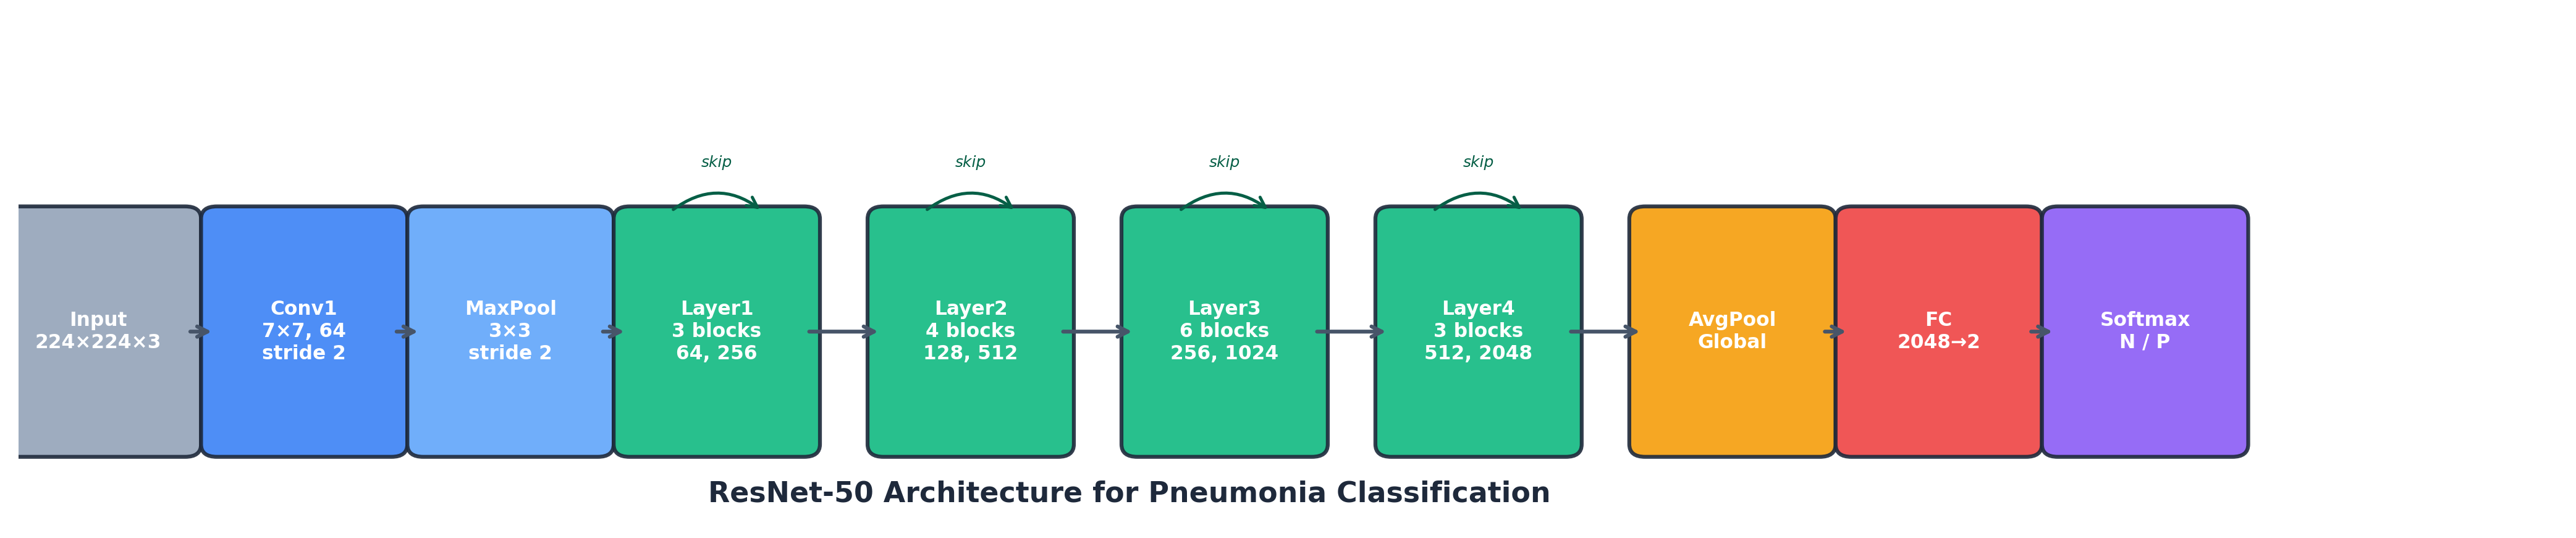
\includegraphics[width=\linewidth]{architecture}
  \caption{High-level overview of the ResNet--50 architecture used in this work. The final fully connected layer is replaced for binary classification.}
  \Description{Block diagram showing the ResNet-50 architecture from input through convolutional blocks with identity connections to the final classification layer.}
  \label{fig:architecture}
\end{figure}

\subsection{Training Strategy}
\label{sec:training}
The model is initialised with ImageNet pre-trained weights. All backbone layers are frozen and only the replacement fully connected layer is trained, constituting a feature-extraction transfer-learning approach. We use cross-entropy loss with class weights inversely proportional to class frequencies to compensate for class imbalance, assigning higher weight to the minority \texttt{Normal} class. The Adam optimiser~\cite{Kingma2015} is configured with a learning rate of $1 \times 10^{-2}$, batch size of 32 and default momentum parameters ($\beta_1 = 0.9$, $\beta_2 = 0.999$). Training is performed for up to 10 epochs with early stopping triggered if the validation loss fails to improve for three consecutive epochs (patience = 3). The model checkpoint with the lowest validation loss is saved as the final model.

\subsection{Interpretability}
\label{sec:interpretability}
To enhance clinical trust, we employ Grad-CAM~\cite{Selvaraju2017} to generate localisation heatmaps indicating the regions that contribute most to the classification decision. Specifically, we hook into the final convolutional block (\texttt{layer4[-1]}) of ResNet--50, compute the gradient of the target class score with respect to the feature maps, and produce a weighted combination that is upsampled and overlaid on the original CXR. By providing these visual explanations, clinicians can confirm that the model focuses on lung fields and opacity regions, improving acceptance of the AI tool.

%% ===========================================================================
\section{Results}
We evaluate the trained model on the held-out test set comprising 624 images (234 Normal, 390 Pneumonia).

\subsection{Quantitative Results}
Table~\ref{tab:metrics} summarises the key performance metrics. The model achieves an overall accuracy of 86.70\% with a recall (sensitivity) of 96.67\% for the pneumonia class, which is clinically desirable as it minimises missed diagnoses. The AUC-ROC of 0.94 indicates strong discriminative ability across classification thresholds.

\begin{table}[t]
  \caption{Test set performance metrics.}
  \label{tab:metrics}
  \begin{tabular}{lcccc}
    \toprule
    Class & Precision & Recall & F$_1$ & Support \\
    \midrule
    Normal    & 0.93 & 0.70 & 0.80 & 234 \\
    Pneumonia & 0.84 & 0.97 & 0.90 & 390 \\
    \midrule
    Accuracy      & \multicolumn{3}{c}{0.87} & 624 \\
    Macro avg     & 0.88 & 0.83 & 0.85 & 624 \\
    Weighted avg  & 0.87 & 0.87 & 0.86 & 624 \\
    \bottomrule
  \end{tabular}
\end{table}

Figure~\ref{fig:confusion} shows the confusion matrix, revealing 164 true negatives, 377 true positives, 70 false positives and 13 false negatives. The low false-negative count (13 out of 390) confirms that the weighted loss successfully prioritises sensitivity, a critical property for a screening tool.

\begin{figure}[t]
  \centering
  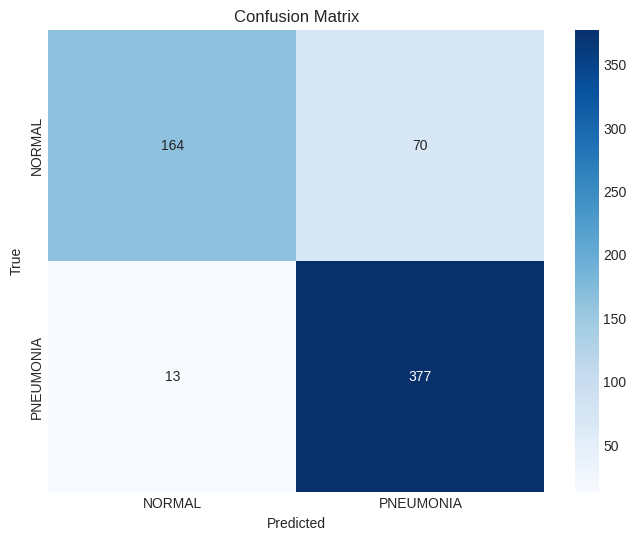
\includegraphics[width=0.85\linewidth]{confusion_matrix}
  \caption{Confusion matrix on the test set. The model achieves high sensitivity (96.67\%) with a modest false-positive rate.}
  \Description{A 2x2 confusion matrix heatmap showing 164 true negatives, 70 false positives, 13 false negatives, and 377 true positives.}
  \label{fig:confusion}
\end{figure}

Figure~\ref{fig:roc} presents the ROC curve with an AUC of 0.94, demonstrating that the model maintains a favourable trade-off between sensitivity and specificity across a range of decision thresholds.

\begin{figure}[t]
  \centering
  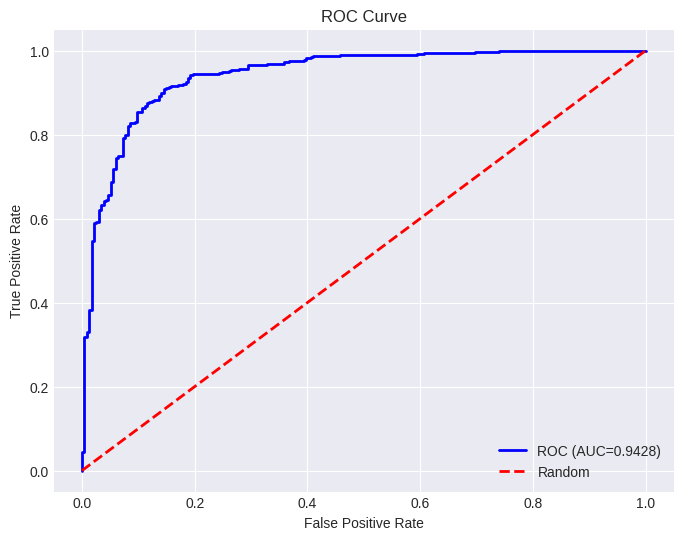
\includegraphics[width=0.85\linewidth]{roc_curve}
  \caption{Receiver operating characteristic (ROC) curve demonstrating the trade-off between sensitivity and specificity (AUC = 0.94).}
  \Description{ROC curve plotting true positive rate against false positive rate, showing an AUC of 0.9428.}
  \label{fig:roc}
\end{figure}

\subsection{Training Dynamics}
Figure~\ref{fig:training} shows the training and validation loss and accuracy across epochs. The model converges rapidly due to the frozen backbone, with early stopping triggered after epoch 5 when validation loss plateaus.

\begin{figure}[t]
  \centering
  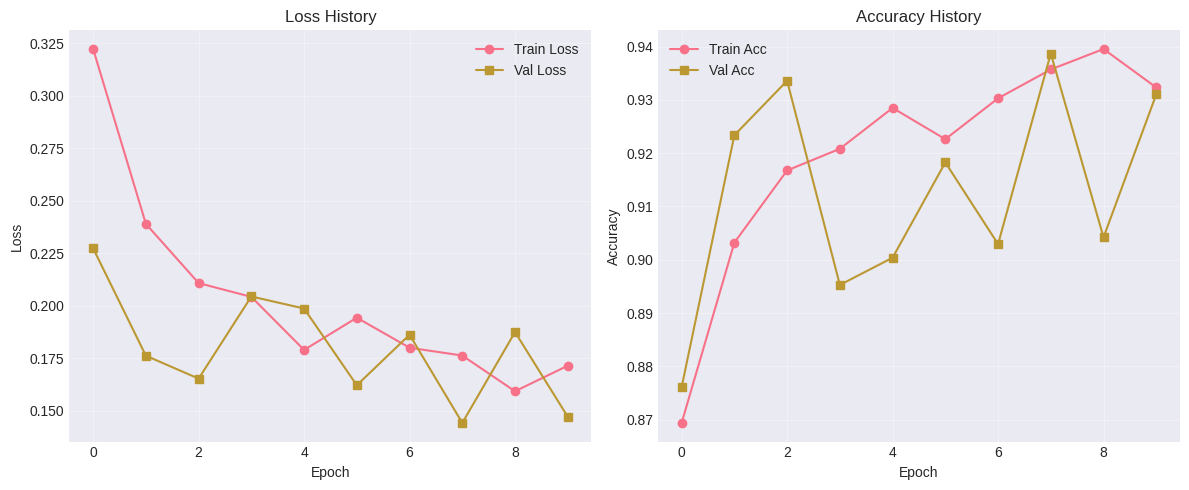
\includegraphics[width=\linewidth]{training_history}
  \caption{Training and validation loss and accuracy across epochs. Early stopping is triggered after minimal improvement.}
  \Description{Two line plots showing training and validation loss decreasing and accuracy increasing over epochs, with early stopping around epoch 5.}
  \label{fig:training}
\end{figure}

\subsection{Qualitative Analysis}
Grad-CAM attention maps confirm that the model attends to anatomically plausible regions. Figure~\ref{fig:gradcam} shows representative heatmap overlays for correctly classified images, where the model focuses on pulmonary fields and opacity regions. Error analysis reveals that misclassifications often correspond to borderline cases with subtle infiltrates or atypical positioning.

\begin{figure}[t]
  \centering
  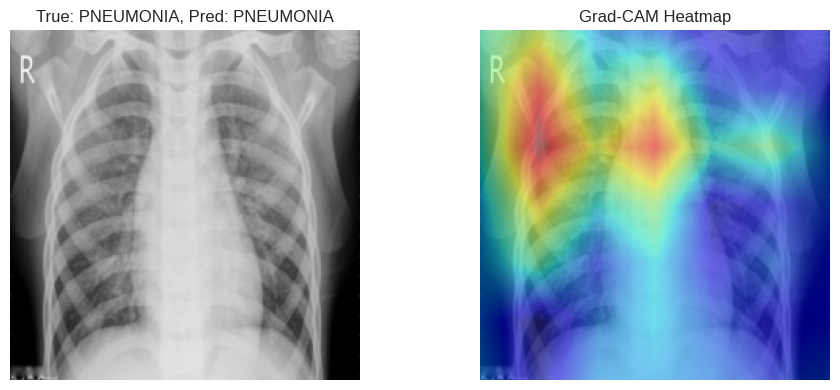
\includegraphics[width=\linewidth]{gradcam_1}
  \caption{Grad-CAM heatmap overlay on correctly classified pneumonia cases, showing the model attends to relevant lung opacity regions.}
  \Description{Chest X-ray images with Grad-CAM heatmap overlays highlighting regions of pneumonia opacities in the lung fields.}
  \label{fig:gradcam}
\end{figure}

%% ===========================================================================
\section{Real-World Application}
We envision integrating the proposed system into a clinical decision support workflow. Patient CXRs are uploaded to a cloud or edge server hosting the ResNet--50 model. The server returns class probabilities and Grad-CAM visualisations via a secure API. Radiologists can use the tool as a second opinion, rapidly triaging normal cases and flagging likely pneumonia for further review.

For settings with limited connectivity, the model can be deployed on an edge device attached to the X-ray machine to provide instant results without requiring a remote server. Key considerations for deployment include data privacy, regulatory compliance (such as adherence to medical device regulations) and continuous monitoring for demographic biases and dataset drift.

%% ===========================================================================
\section{Future Work}
To evolve this prototype into a clinically viable software as a medical device (SaMD), future work will focus on:

\begin{itemize}
  \item \textbf{Data diversity:} Augmenting the dataset with images from diverse demographics and adult populations to mitigate demographic bias, as the current dataset is restricted to paediatric patients from a single centre.
  \item \textbf{Fine-tuning the full network:} Unfreezing deeper layers with a discriminative learning rate schedule to improve feature adaptation beyond ImageNet representations.
  \item \textbf{Multi-class classification:} Extending the model to distinguish bacterial, viral and atypical pneumonia sub-types and to provide severity grading.
  \item \textbf{Data augmentation:} Incorporating random rotations, horizontal flips and intensity jittering to improve generalisation and robustness.
  \item \textbf{Ensemble methods:} Combining multiple architectures (e.g., DenseNet, EfficientNet) to improve robustness and calibration.
  \item \textbf{Regulatory compliance:} Ensuring adherence to medical device regulations and ethical considerations such as fairness and explainability.
\end{itemize}

%% ===========================================================================
\section{Conclusion}
We have presented an automated pneumonia screening system leveraging transfer learning with ResNet--50 and interpretability via Grad-CAM. The system effectively classifies chest X-rays into normal and pneumonia classes, achieving 86.70\% accuracy, 96.67\% recall and an AUC-ROC of 0.94 on the benchmark dataset. By addressing class imbalance through weighted loss functions, incorporating early stopping and providing visual explanations, the model demonstrates potential for deployment as a decision support tool in resource-constrained healthcare environments. Ongoing work will expand the dataset, explore full network fine-tuning and extend the model to more granular classification tasks, paving the way for clinically useful AI-driven diagnostic aids.

%% ===========================================================================
\bibliographystyle{ACM-Reference-Format}
\bibliography{references}

\end{document}
